



Waves are usually the first type of motion that you see at the sea surface, and they appear in all remotely sensed data. In some cases, the direct wave influence can be averaged out of the signal. In other cases there is a residual bias due to the presence of waves. This is the case in 
range measurements with altimeters \citep[e.g.][]{Minster&al.1992}, velocity measurement with Doppler systems
\citep{Chapron&al.2005,Nouguier&al.2018}, surface brighness temperature measurements used to infer 
sea surface temperature or salinity \citep{Reul&Chapron2003}. Wave shapes and motion also introduce a variance in the 
measured quantity which can be useful in the case of sea level measurement with altimetry, or can blur 
the signal beyond recognition in SAR imagery or interferometry \citep{Peral&al.2015}. All these effects are opportunities for measuring wave parameters, or measuring other processes thanks to their influence on waves. 

\section{Back-scatter from a rough surface}
The patterns observed on the sea surface depend on the surface properties (slopes, velocities, whitecaps ...) but also on the viewing geometry and on instrument parameters (electromagnetic wavelength polarization) and on processing details (real aperture, synthetic aperture ...), it is thus difficult to give a comprehensive accounts of the many different looks that the same piece of ocean can have. 


%%%%%%%%%%%%%%%%%%%%%%%%%%%%%%%%%%%%%%%%%%%%%%%%%%%%%%%%%%%%%%%%%%%%%%%%%%%%%%%%%%
\begin{figure}[htb]
\centerline{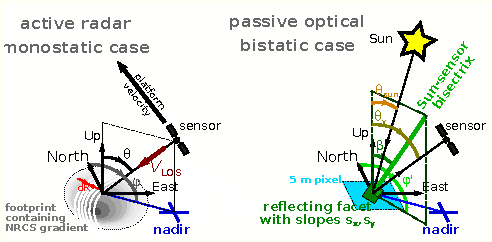
\includegraphics[width=0.6\linewidth]{FIGS_CH_REMOTE/geometry_optical.pdf}}
% note that the square brace option below is only required
% if you intend to produce a list of illustrations
% THIS FIGURE WILL BE A FULL PAGE LANDSCAPE
\caption[]
{Two typical examples of observation geometry of the ocean. Left: observation with a radar looking sideways, the radar is both the source and the receiver of the signal, this is a monostatic measuremnt with ocean apparent properties determined by the incidence angle $\theta_v$ and azimuth of the line of sight, as well as radar wavelength and polarization. Right: observation of the sun reflection of the sea surface. Here, for this bistatic geometry, the important direction is not the line of sight but the direction of the sun-sensor bisectrix. \label{fig:remote_sensing_geometry}}
\end{figure}
%%%%%%%%%%%%%%%%%%%%%%%%%%%%%%%%%%%%%%%%%%%%%%%%%%%%%%%%%%%%%%%%%%%%%%%%%%%%%%%%%%
For electromagnetic wavelengths much shorter than the shortest waves (a few millimeters), the ocean surface is locally smooth and the reflection can be completely described by geometrical optics: we can decompose the sea surface in elementary "facets" that are locally flat and reflect the light in the specular direction. 


When looking in the sun glitter,  the apparent brightness of the the ocean depends on the probability that the piece of ocean considered (a "pixel") contains the slope that corresponds to a bistatic reflector of the sun. For pixels smaller than a few hundreds of meters, the brightness of these pixels fluctuates due to the finite number of "specular points" \citep{Longuet-Higgins1960c}. 

A first good approximation for the slope PDF is that it follows a Guassian distribution for the two dimensions that are the slopes $s_x=\partial \zeta / \partial x$ and $s_y=\partial \zeta / \partial y$ along the $x$ and $y$ directions. In this section we will now choose to have the $x$ direction  in the wind direction. Under this Gaussian approximation the slope PDF is completely determined by slopes variances $\mathrm{mss}_x=\left< s_x^2 \right>$ and $\mathrm{mss}_y=\left< s_y^2 \right>$ as, 
\begin{equation}
p(s_x,s_y) \simeq p_G(s_x,s_y)=\frac{1}{2 \pi \sqrt{\mathrm{mss}_x \mathrm{mss}_y} } \exp \left[-\frac{1}{2} \left(\frac{s_x^2}{\mathrm{mss}_x} + \frac{s_y^2}{\mathrm{mss}_y}\right)\right].
\end{equation}

For moderate wind speeds, $\mathrm{mss}_x \simeq \mathrm{mss}_y \simeq \mathrm{mss}/2$ and the slope distribution further simplifies as an isotropic function that is completely defined by the total mean square slope mss=$\mathrm{mss}_x +\mathrm{mss}_y$, 
\begin{equation}
p(s_x,s_y) \simeq p_{G,\mathrm{iso}}(s_x,s_y)=\frac{1}{ \pi \mathrm{mss}} \exp \left[- \frac{s_x^2+s_y^2}{\mathrm{mss}}\right].
\end{equation}


All measurements, pioneered by \cite{Cox&Munk1954} and confirmed by \cite{Breon&Henriot2006}, have shown that the variances of crosswind and downwind slopes grow linearly with the wind speed, as shown in figure \ref{fig:slope_pdf}.a, with a faster growth of the downwind slopes. The total mean square slope (mss) is the sum of these two components, with a value around 0.029 for a wind speed of 5 m/s, corresponding to a root mean square slope of 0.17, or an angle of the sea surface of 10 degrees relative to the horizontal. In practice the mss also varies with the state of development of the wind sea, by up to  20\% \citep[$\pm 1~dB$ in][]{Nouguier&al.2016}, and the presence of current gradients, by about 10\% \citep[e.g.][]{Rascle&al.2017}. The largest local changes in mss are associated to the presence of oily films at the sea surface that can strongly damp the shortest wave components. 

%%%%%%%%%%%%%%%%%%%%%%%%%%%%%%%%%%%%%%%%%%%%%%%%%%%%%%%%%%%%%%%%%%%%%%%%%%%%%%%%%%
\begin{figure}[htb]
\centerline{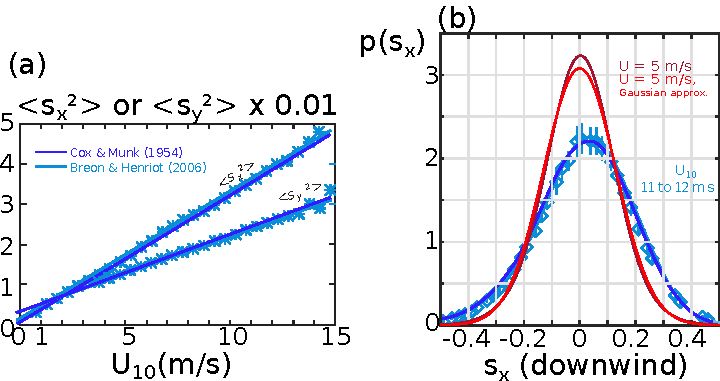
\includegraphics[width=0.7\linewidth]{FIGS_CH_REMOTE/slope_pdf.pdf}}
% note that the square brace option below is only required
% if you intend to produce a list of illustrations
% THIS FIGURE WILL BE A FULL PAGE LANDSCAPE
\caption[]
{(a) variation of the downwind and crosswind slope varianace with wind speed. (b) example of slope PDF for a given mean square slope, corresponding to a widn speed of 5 m/s or in the range 11 to 12 m/s. Adapted from Munk (2009) \label{fig:slope_pdf}}
\end{figure}
%%%%%%%%%%%%%%%%%%%%%%%%%%%%%%%%%%%%%%%%%%%%%%%%%%%%%%%%%%%%%%%%%%%%%%%%%%%%%%%%%%

For a given slope (or view direction), the PDF (or image brightness) changes if the mss changes. In figure \ref{fig:slope_pdf}.b, the PDF increases for small slopes when the mss drops from 0.06 (for 11.5 m/s wind) to 0.03 (for 5 m/s wind, or for higher winds but in the presence of surface slicks), and it decreases for larger slopes. 
 Hence the contrast in the sun reflection in an optical or radar image depends 
on viewing geometry: near the center of the sun glint (or near the vertical for a monostatic radar) a slick flat surface will appear bright, but it will be dark away from the center (at higher incidences for a monostatic radar) as shown in the photograph in figure \ref{fig:slicks} for a bistatic viewing geometry.
%%%%%%%%%%%%%%%%%%%%%%%%%%%%%%%%%%%%%%%%%%%%%%%%%%%%%%%%%%%%%%%%%%%%%%%%%%%%%%%%%%
\begin{figure}[htb]
\centerline{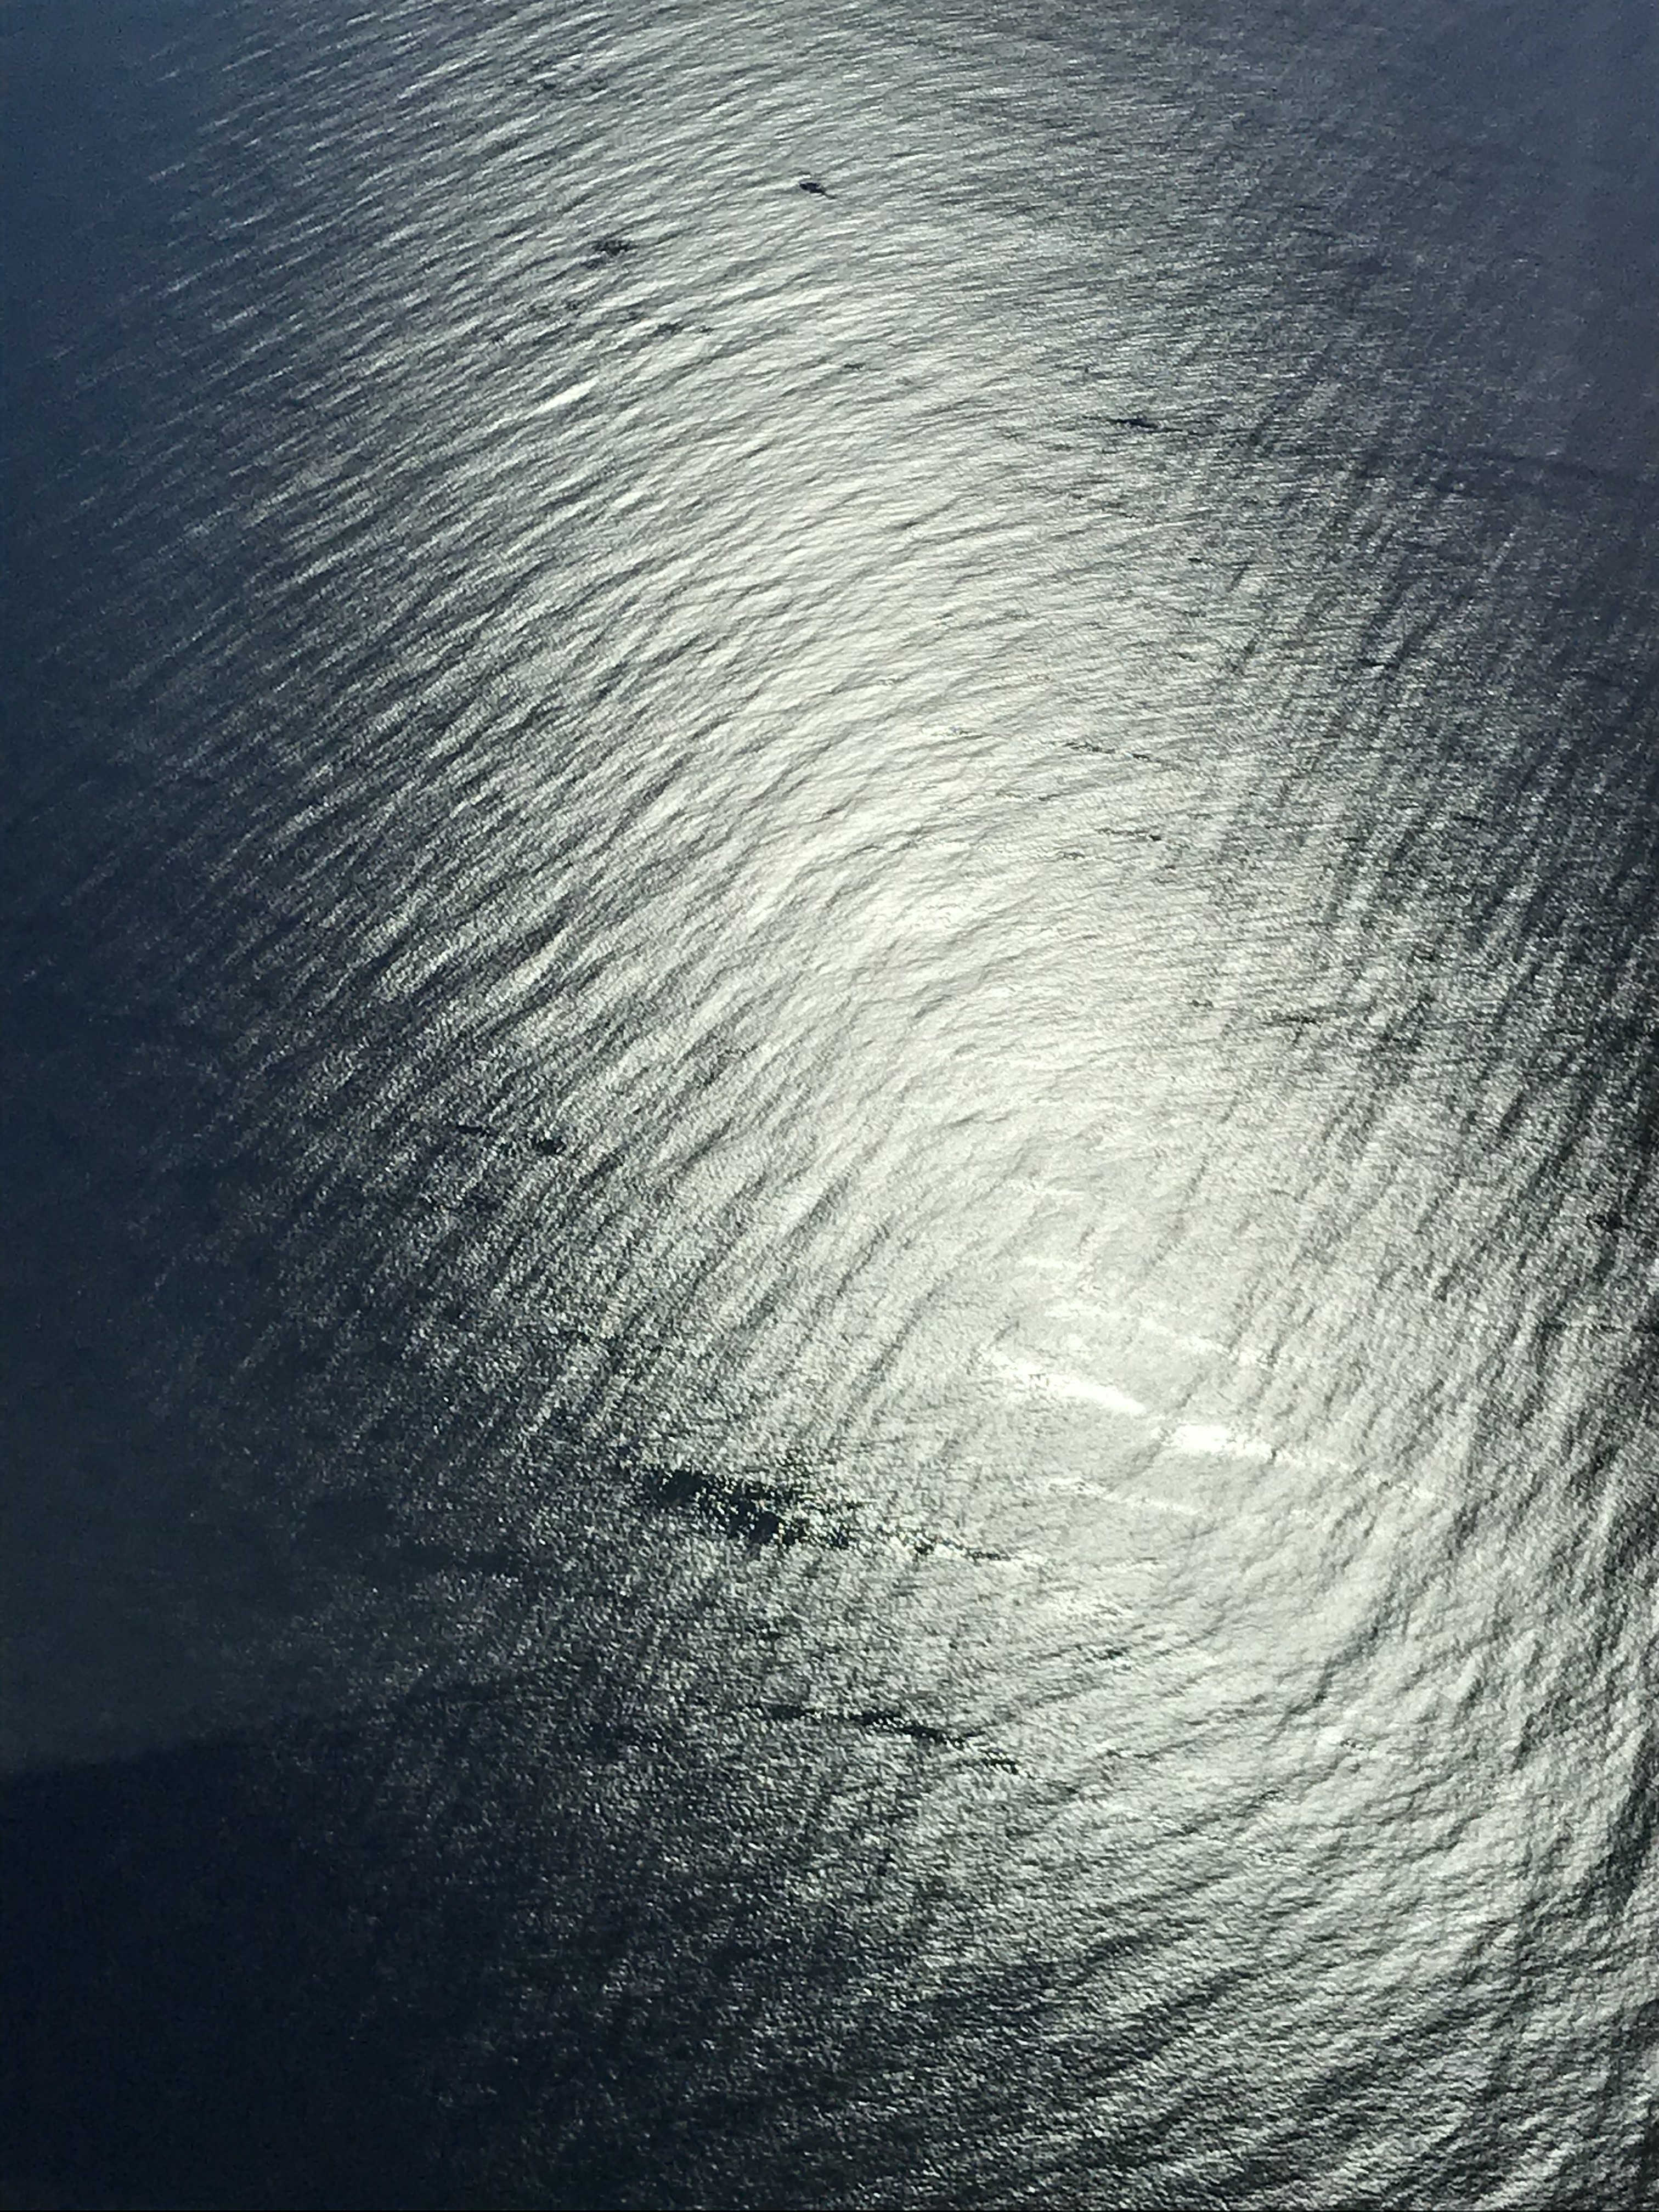
\includegraphics[width=0.6\linewidth]{FIGS_CH_REMOTE/glitter_and_slicks_small.jpeg}}
% note that the square brace option below is only required
% if you intend to produce a list of illustrations
% THIS FIGURE WILL BE A FULL PAGE LANDSCAPE
\caption[]{A view of the ocean from an aircraft, looking at the sun reflection: locally the ocean surface is made smooth by the presence of surface material that makes the sea smooth. When this happens near the center of the sun glint, the image is brighter, when this is away from the center of the sun glint, the ocean appears darker. Image taken in the Californial bight by Luc Lenain. \label{fig:slicks}}
\end{figure}
%%%%%%%%%%%%%%%%%%%%%%%%%%%%%%%%%%%%%%%%%%%%%%%%%%%%%%%%%%%%%%%%%%%%%%%%%%%%%%%%%% 

The Gaussian approximation can be corrected with a Gram-Charlier expansion based on the measurement of various statistical  moments of the slope PDF, including the mean, which is not zero, as well as the asymetry and skewness of the waves \citep{Cox&Munk1954,Munk2009}. Fig. \ref{fig:slope_pdf}.b shows that for low wind speeds, non-Gaussian effects mostly introduce a larger probability of near-zero slopes and high slopes, but little change of the probability around $s_x=\mathrm{mss}_x$. These can be associated to nonlinear Stokes-type corrections to the linear wave profile. At higher wind speeds, the asymetry becomes significant, and the most likely surface slope is not at zero, but at slightly positive value of $\partial \zeta/ \partial x$ that corresponds to the larger area of the (positively sloping: $\partial \zeta/ \partial x > 0$) rear face of the waves compared to the (negatively sloping) front face of the waves, the latter being steeper and shorter. 

In the case of visible light,  the diffuse light source from the blue sky and clouds must be taken into account for large values of $\beta$, and at night the moon can be used instead of the sun. 

For longer eletromagnetic wavelenghts, i.e. all main active radar bands used in ocean remote sensing from Ka band (8 mm wavelength) to L band (20 cm or so), the active radar can generally be considered to be the sole source of radiation, although that could change with 5G mobile phones infringing on the Ka-band. %Other sources of L-band radiation include hydrogen clouds (in particular in our galaxy) that are an important source of signals picked up by the passive radiometers on SMOS, but generally much weaker than 
 The surface is rough for microwave radiation, although specular reflection is still relevant at near-nadir viewing angles, particularly strong reflection occurs when the phases of the surface topography combine constructively with the phases of the incident radar waves: this is Bragg scattering and it typically explains most of the reflections at large incidence angles $\theta_v$.

\subsection{near-nadir incidences}
For near-vertical angles the power recorded on a radar is well described by the theory for a nearly Gaussian distribution of surface slopes, 
completely determined by the mss. In general, the mss is largely determined by the wind speed, but it is also modified by the stage of  development of the wave field, increasing for more mature waves that generally correspond to higher wave heights, as shown in figure 
\ref{fig:sigma0}.b. 

%%%%%%%%%%%%%%%%%%%%%%%%%%%%%%%%%%%%%%%%%%%%%%%%%%%%%%%%%%%%%%%%%%%%%%%%%%%%%%%%%%
\begin{figure}[htb]
\centerline{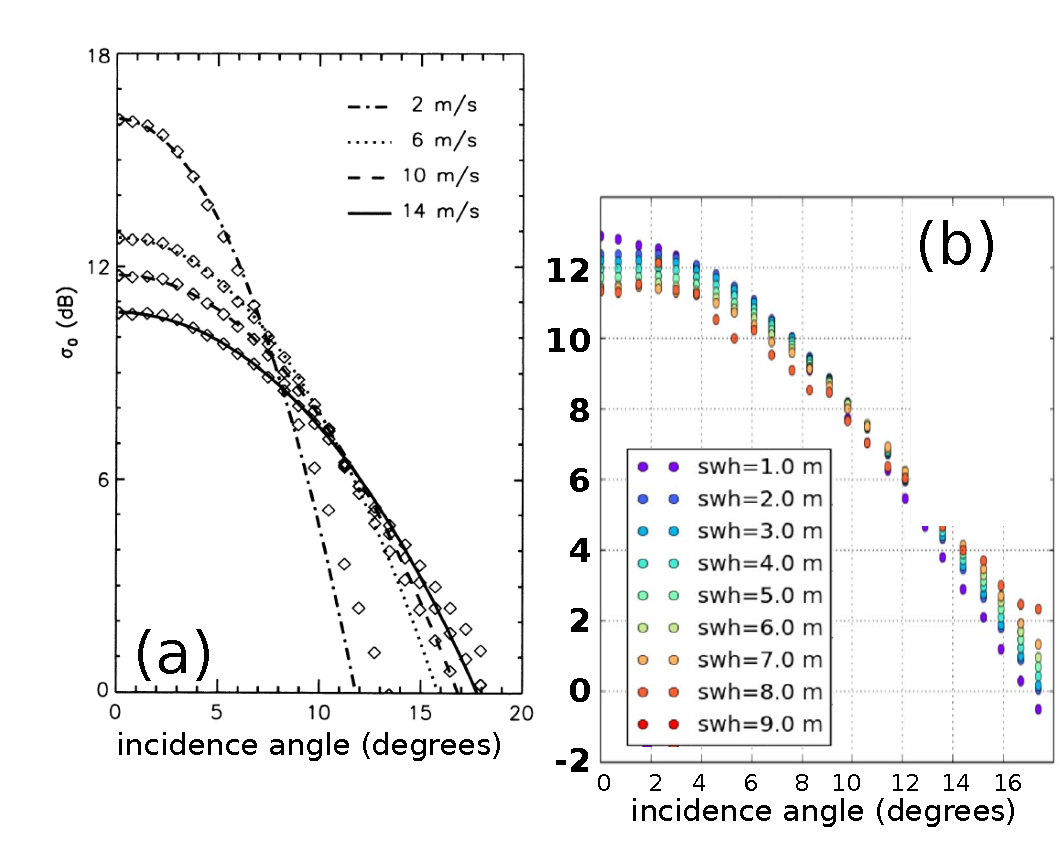
\includegraphics[width=0.6\linewidth]{FIGS_CH_REMOTE/sigma0.pdf}}
% note that the square brace option below is only required
% if you intend to produce a list of illustrations
% THIS FIGURE WILL BE A FULL PAGE LANDSCAPE
\caption[Radar return power in Ku-band as a function of wind speed, incidence angle and sea state]
{(a) Average backscatter power from the TRMM radar \citep[from][]{Freilich&Vanhoff2003} 
(b) Same variation for a given wind speed, as a function of wave height \citep[from][]{Nouguier&al.2016}. \label{fig:sigma0}}
\end{figure}
%%%%%%%%%%%%%%%%%%%%%%%%%%%%%%%%%%%%%%%%%%%%%%%%%%%%%%%%%%%%%%%%%%%%%%%%%%%%%%%%%%




A flat surface gives a strong return near zero incidence (vertical sounding) and the return power decreases as $1/$mss. For incience angles 
larger than about 10$^\circ$ in Ku-band, the return increases with the roughness.


\subsection{higher incidence angle}
For large incidence angles the reflection is proportional to the amplitude of waves in the radar look direction and with a wavelength 
equal to $\lambda_e / (2 \sin \theta_i)$ where $\lambda_e$ is the electromagnetic wavelength. These waves are called 'Bragg waves'. A similar 
scattering of waves by a periodic medium was described by \cite{Bragg1913} in the case of X-ray diffraction, and is thus known as Bragg scattering, although it 
was first studied by \cite{Rayleigh1896} for the reflection of sound waves at a wavy surface. This generally applies to incidence angles above 30$^\circ$, and 
is used in the remote sensing of winds with ``scatterometers'' as well as the measurement of currents with HF-radars having wavelength of several meters and using 
grazing incidence angles (close to 90$^\circ$). 

\section{Various applications}
\subsection{Roughness and surface current gradients}
Waves with wavelengths under 3~m are the main contribution to the surface slope variance \citep[e.g.][]{Cox&Munk1954,Vandemark&al.2002}, and 
these short waves are strongly modified by current gradients \citep[e.g.][]{Phillips1984}. As a result, current gradients have a clear signature in the mean 
square slopes and the measured back-scatter intensity for incidences 0 to 20$^\circ$, as shown in figure \ref{fig:glint}. 
%%%%%%%%%%%%% figure
\begin{figure}
\centerline{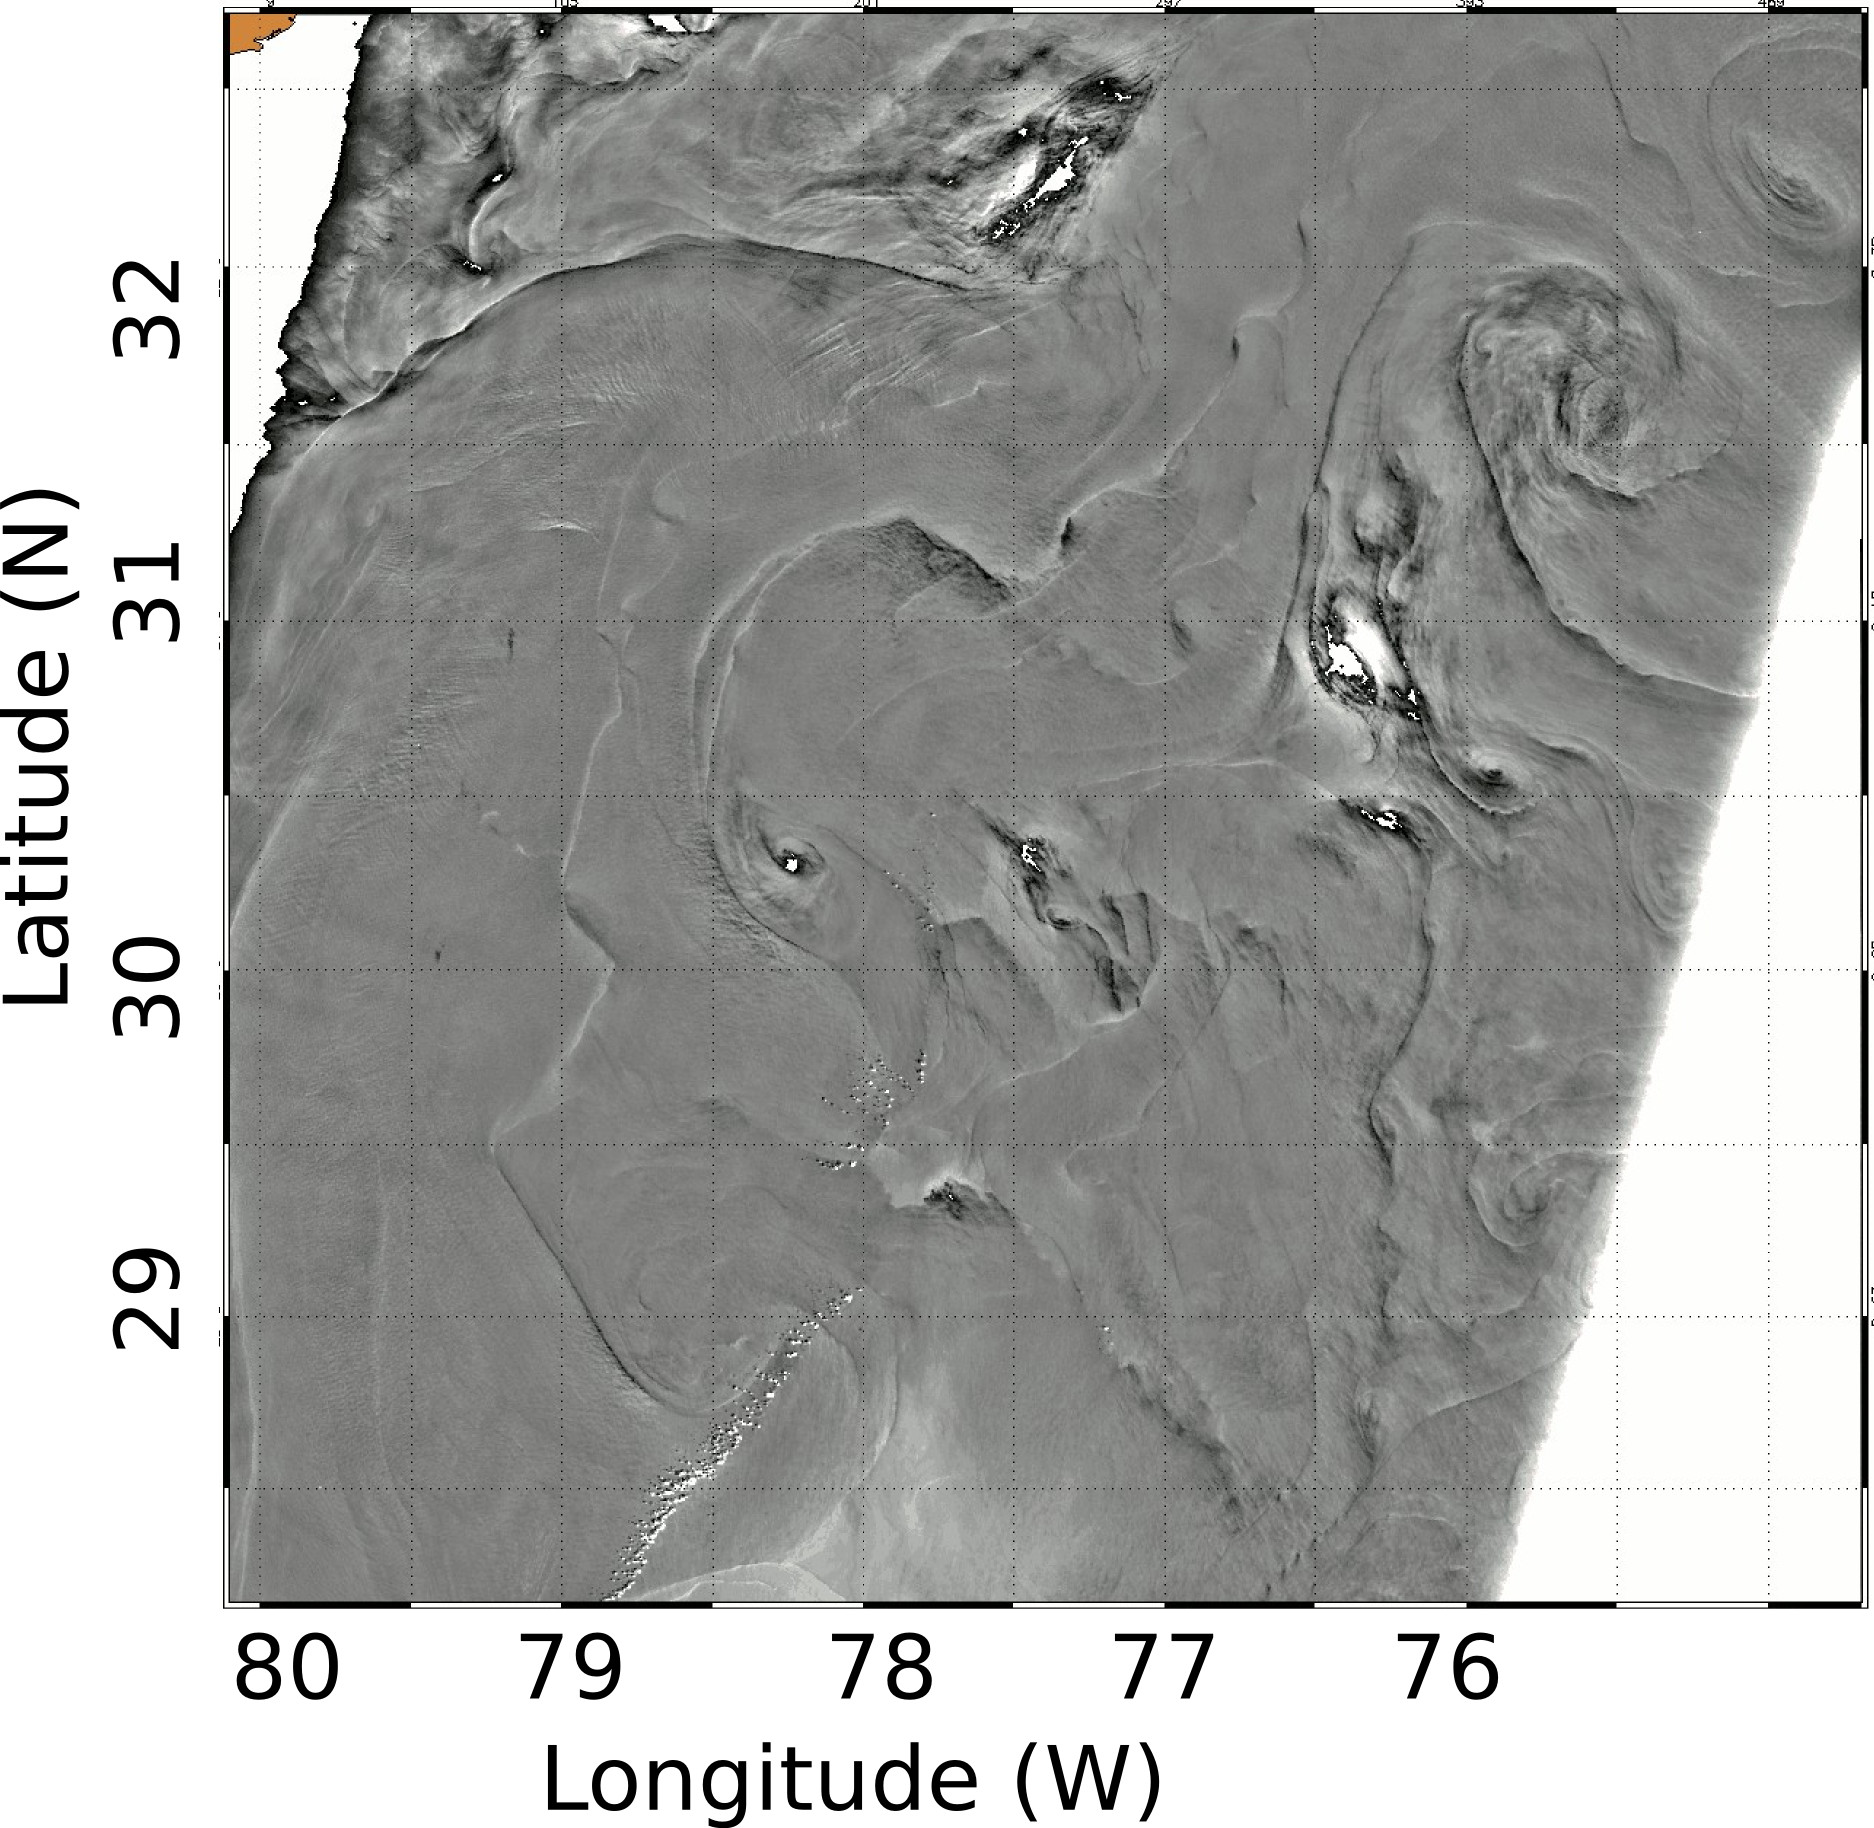
\includegraphics[width=0.8\textwidth]{FIGS_CH_REMOTE/sun_glint.jpg}}
  \caption{Surface roughness observed by the MERIS instrument on board ENVISAT.}
  \label{fig:glint}
\end{figure}
%%%%%%%%%%%%% end of figure
This property has been particularly investigated by 
\cite{Kudryavtsev&al.2012,Rascle&al.2014,Rascle&al.2017}, with the objective of estimated current gradients from optical imagery in the 'sun glint', i.e. 
for incidence angles close to the specular reflection direction of the sun.  The quantitative analysis of glint data is generally based on the wave action equation 
as given in chapter \ref{ch_current}.

